Knot theory is a centuries-old field of study. A knot in mathematics is much like a knot in the real world: a string looped around itself without being torn apart. In mathematics, we require the two ends of the string to be "glued" together. A knot is therefore like a tangled circle. We define a knot formally below.
\begin{definition}[Knot]
A \emph{knot} is an embedding of the circle, $S^1$, in $\mathbb{R}^3$.\\\\
We say $S^1$ is \emph{embedded} in $\mathbb{R}^3$ if there is an injective, continuous map $f:S^1 \rightarrow \mathbb{R}^3$ such that $f(S^1)$, a subspace of $\mathbb{R}^3$ with the subspace topology, is homeomorphic to $S^1$.
\end{definition}

\begin{remark}
Knots can be visualized in two-space with a \emph{knot diagram}. Knot diagrams show where the knot crosses over itself. Knots are named according to the number of crossings in their knot diagram. In the third example below, the knot crosses itself seven times. Since there are multiple knots with the same number of crossings, knots are assigned an arbitrary subscript. In this case it is 3. Hence the name $7_{3}$.
\end{remark}

The most simple example of a knot is the unknot, which is a loop without tangles.
\begin{figure}[H]
\centering
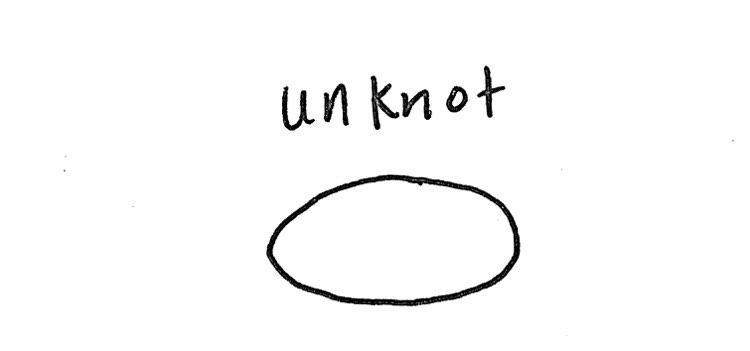
\includegraphics[scale=0.2]{figures/unknot.jpg}
\end{figure}

Another simple example is the trefoil knot.
\begin{figure}[H]
\centering
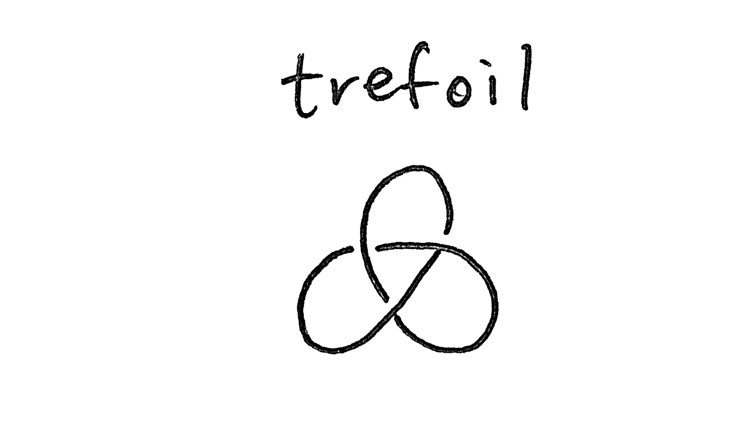
\includegraphics[scale=0.2]{figures/trefoil.jpg}
\end{figure}

Here is a more complicated knot:
\begin{figure}[H]
\centering
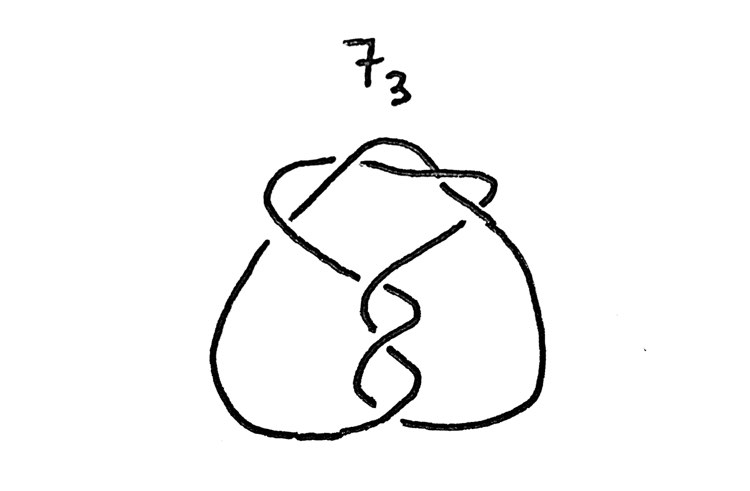
\includegraphics[scale=0.2]{figures/knot73.jpg}
\end{figure}

\noindent Now, how do we know if two knots are the same? We usually consider two spaces equivalent if they are homeomorphic. The spaces $K_1$ and $K_2$ of two knots are always homeomorphic; both spaces are homeomorphic to the circle. We must create a more meaningful definition of knot equivalence.

\noindent In general terms, two knots are equivalent if one can be deformed into the other without tearing it, eg, without passing it through itself. Formally,

\begin{definition}[Knot Equivalence]
Two knots $K_1$ and $K_2$ in $\mathbb{R}^3$ are \eph{equivalent} if there is a homeomorphism $f$ between $\mathbb{R}^3$ and itself such that $f(K_1) = K_2$.
\end{definition}

\noindent Now we introduce an object that will help us determine knot equivalence.
\begin{definition}[Knot Group]
The knot group of a knot $K$ is the fundamental group of $\mathbb{R}^3\setminus{K}$.
\end{definition}
\noindent The knot group is a knot invariant, meaning that equivalent knots have isomorphic knot groups. The contrapositive of this statement is that two knots are different if their knot groups are different. This means we can use knot groups to figure out if two knots are different.